


\vspace{-4pt}
\section{Experiments}

\vspace{-4pt}
\subsection{Simulation Evaluation}
\vspace{-2pt}

\begin{table*}[t]
\centering
\small
\resizebox{\textwidth}{!}{
\begin{tabular}{l|*{3}{c}|*{4}{c}|*{2}{c}|c}
\toprule
  & \multicolumn{3}{c|}{Adroit} & \multicolumn{4}{c|}{DexArt} & \multicolumn{2}{c|}{MetaWorld} &  \\
 Method & Hammer & Door & Pen & Laptop & Faucet & Toilet & Bucket & Medium (6) & Hard (5) & Success \\
\midrule
IBC & \dd{0.00}{0.00}  & \dd{0.00}{0.00} & \dd{0.10}{0.01} & \dd{0.01}{0.01} & \dd{0.07}{0.02} & \dd{0.15}{0.01} & \dd{0.00}{0.00} & \dd{0.11}{0.02} & \dd{0.09}{0.03} & 0.08  \\
 BC-H & \dd{0.10}{0.09}  & \dd{0.07}{0.05} & \dd{0.16}{0.03} & \dd{0.09}{0.02} & \dd{0.13}{0.04} & \dd{0.21}{0.02} & \dd{0.10}{0.01} & \dd{0.15}{0.03} & \dd{0.18}{0.05} & 0.15 \\
DP & \dd{0.48}{0.17}  & \dd{0.50}{0.05} & \dd{0.25}{0.04} & \dd{0.69}{0.04} & \dd{0.23}{0.08} & \dd{0.58}{0.02} & \dd{0.46}{0.01} & \dd{0.20}{0.05} & \dd{0.19}{0.03} & 0.30  \\
DP3 & \ddbfgreen{1.00}{0.00} & \dd{0.62}{0.04} & \dd{0.43}{0.06} & \dd{0.83}{0.01} & \dd{0.63}{0.02} & \ddbfgreen{0.82}{0.04} & \dd{0.46}{0.02} & \dd{0.45}{0.05} & \dd{0.35}{0.02} & 0.51  \\
FlowPolicy & \ddbfgreen{1.00}{0.00} & \dd{0.58}{0.05} & \dd{0.53}{0.12} & \dd{0.85}{0.02} & \dd{0.42}{0.10} & \dd{0.80}{0.05} & \dd{0.39}{0.06} & \dd{0.47}{0.07} & \dd{0.37}{0.07} & 0.51   \\
\textbf{\mymethod{} (Ours)} & \ddbfgreen{1.00}{0.00} & \ddbfgreen{0.65}{0.03} & \ddbfgreen{0.65}{0.01} & \ddbfgreen{0.90}{0.02} & \ddbfgreen{0.72}{0.05} & \ddbfgreen{0.82}{0.02} & \ddbfgreen{0.47}{0.02} & \ddbfgreen{0.68}{0.04} & \ddbfgreen{0.72}{0.03} & {\cellcolor{tablecolor2}$\mathbf{0.72}$}  \\
\bottomrule
\end{tabular}
\vspace{-24pt}
}
\caption{Quantitative comparison of \mymethod{} against state-of-the-art baselines on 18 tasks from three simulation benchmarks.
}
\vspace{-8pt}
\label{tab:sim}
\end{table*}


% \subsection{Benchmarks and Datasets}

\textbf{Benchmarks and Datasets. }We evaluate our method on manipulation benchmarks that cover a broad range of control domains. We use Adroit~\citep{rajeswaran2017learning}, DexArt~\citep{bao2023dexart} and MetaWorld~\citep{yu2020meta} as our simulation benchmarks. These are implemented on physics engines like MuJoCo~\citep{todorov2012mujoco} and IsaacGym~\citep{makoviychuk2021isaac}. For fair comparison we adopt the same task splits and data collection pipelines as in prior work~\citep{ze20243d}: Adroit tasks with high-dimensional Shadow hand and MetaWorld with low-dimensional gripper are trained with 10 expert demos per task, while DexArt with Allegro hand uses 90 expert demos. Demonstrations are collected using scripted policies for MetaWorld tasks, and RL-trained expert agents~\citep{wang2022vrl3, schulman2017proximal} for Adroit and DexArt. Each experiment is run with three random seeds. For each seed we evaluate the policy for 20 episodes every 200 training epochs and then compute the average of the top-5 highest success rates~\citep{ze20243d}. The final metric is the mean and standard deviation across the three seeds. 

\textbf{Experiment Setup. } All networks are optimized with AdamW~\citep{loshchilov2017decoupled}. We apply a short linear warmup followed by cosine decay for the learning rate. Training proceeds in stages: first we pretrain the VQ-VAE to learn compact primary prototypes; then we freeze the codebook and jointly train the Primary Mode Policy $\pi_1$ (cross-entropy to the VQ indices) and the mode-conditioned MeanFlow generator $\bar v_\theta$ (squared-error supervision on sampled $(\tau,r)$ intervals). At inference we set $(\tau,r)=(0,1)$ for one-step continuous action chunk generation.

% \subsection{Baselines}

\textbf{Baselines. }We compare against the following representative baselines. 
Implicit Behavioral Cloning (IBC)~\citep{florence2022implicit} serves as a representative implicit BC method. 
BC-H~\citep{foster2024behavior} represents non-generative approaches for mitigating mode instability.
Diffusion Policy (DP)~\citep{chi2023diffusion} pioneers the original formulation of image-conditioned diffusion-based policies. While 3D Diffusion Policy (DP3)~\citep{ze20243d} represents a recent advancement in 3D-point-cloud conditioned diffusion-based policies, Flow Policy (FP)~\citep{zhang2025flowpolicy} falls into the category of normalizing-flow-based policy variants.  These baselines provide a spectrum from energy-based model to expressive generative policies.


\textbf{Key Findings. }Across Adroit, DexArt and MetaWorld, our method substantially outperforms diffusion and other baselines. 
Table~\ref{tab:sim} highlights our work performance on 18 core tasks, while comprehensive results across all 56 tasks are detailed in Appendix.
Beyond that, our two-stage design preserves primary-mode consistency even when action chunks are short, which approaches closed-loop and highly reactive operation. Meanwhile, our primary-mode tiny MLP and the one-step generator together yield fast generation while maintaining high success rates, as discussed in Ablations section. These findings indicate that explicitly decoupling coarse discrete mode selection from continuous intra-mode variation yields both statistical and practical benefits.


\begin{figure*}[tb]
  \centering
  % \vspace{-8pt}
  
\includegraphics[width=0.99\linewidth]{pics/real_compare.pdf}
  \vspace{-12pt}
  \caption{Visual comparison of failure modes in baselines versus \mymethod. \textbf{Mode Collapse} outputs ``average'' actions, while \textbf{Mode Bouncing} randomly switches between consecutive time steps.
  }
  \vspace{-8pt}
  \label{fig:real_compare}
\end{figure*}

\vspace{-4pt}
\subsection{Real World Evaluation}
\vspace{-2pt}

% \begin{table*}[t]
% \centering
% \small
% \resizebox{\textwidth}{!}{
% \begin{tabular}{l|lccccc|c}
% \toprule
% Method & Task Description & \# Variations & \# Demos & End Effector & Tactile & Action Dim & Success \\
% \midrule
% \multirow{4}{*}{Vanilla BC} & \textit{Pick Cube} & 3 & 50 & Gripper & \no & \(7+1\) & 0.20 \\
% & \textit{Place Baymax} & 1 & 10 & Gripper & \no & \(7+1\) & 0.40 \\
% & \textit{Wipe Table} & 5 & 50 & XHand & \yes & \(7+12\) & 0.00 \\
% & \textit{Place Toy Into Bin} & 4 & 50 & XHand & \yes & \(7+12\) & 0.00 \\
% \midrule
% \multirow{4}{*}{DP3} & \textit{Pick Cube} & 3 & 50 & Gripper & \no & \(7+1\) & 0.60 \\
% & \textit{Place Baymax} & 1 & 10 & Gripper & \no & \(7+1\) & 0.85 \\
% & \textit{Wipe Table} & 5 & 50 & XHand & \yes & \(7+12\) & 0.55 \\
% & \textit{Place Toy Into Bin} & 4 & 50 & XHand & \yes & \(7+12\) & 0.60 \\
% \midrule
% \multirow{4}{*}{\textbf{\mymethod{} (Ours)}} & \textit{Pick Cube} & 3 & 50 & Gripper & \no & \(7+1\) & {\cellcolor{tablecolor2}$\mathbf{0.70}$} \\
% & \textit{Place Baymax} & 1 & 10 & Gripper & \no & \(7+1\) & {\cellcolor{tablecolor2}$\mathbf{0.90}$} \\
% & \textit{Wipe Table} & 5 & 50 & XHand & \yes & \(7+12\) & {\cellcolor{tablecolor2}$\mathbf{0.70}$} \\
% & \textit{Place Toy Into Bin} & 4 & 50 & XHand & \yes & \(7+12\) & {\cellcolor{tablecolor2}$\mathbf{0.80}$} \\
% \bottomrule
% \end{tabular}
% }
% \vspace{-8pt}
% \caption{Quantitative comparison of \mymethod{} and baselines on real-world manipulation tasks}
% \vspace{-16pt}
% \label{tab:real_result}
% \end{table*}




\begin{table*}[t]
\centering
\small
\resizebox{\textwidth}{!}{
\begin{tabular}{l|ccccc|ccc}
\toprule
\multirow{2}{*}{\textit{Task Description}} & \multicolumn{5}{c|}{Task Parameters} & \multicolumn{3}{c}{Success Rate} \\
% \cmidrule(lr){2-6}\cmidrule(lr){7-9}
& \# Variations & \# Demos & End Effector & Tactile & Action Dim & Vanilla BC & DP3 & \textbf{\mymethod{} (Ours)} \\
\midrule
\textit{Pick Cube} & 3 & 50 & Gripper & \no & \(7+1\) & 0.20 & 0.60 & {\cellcolor{tablecolor2}$\mathbf{0.70}$} \\
\textit{Place Baymax} & 1 & 10 & Gripper & \no & \(7+1\) & 0.40 & 0.85 & {\cellcolor{tablecolor2}$\mathbf{0.90}$} \\
\textit{Wipe Table} & 5 & 50 & XHand & \yes & \(7+12\) & 0.00 & 0.55 & {\cellcolor{tablecolor2}$\mathbf{0.70}$} \\
\textit{Place Toy Into Bin} & 4 & 50 & XHand & \yes & \(7+12\) & 0.00 & 0.60 & {\cellcolor{tablecolor2}$\mathbf{0.80}$} \\
\bottomrule
\end{tabular}
}
\vspace{-12pt}
\caption{Quantitative comparison of success rates of different methods on real world manipulation tasks. The table presents key task parameters alongside the performance of each method.}
\vspace{-8pt}
\label{tab:real_result}
\end{table*}




\begin{table}[t]
\centering
\small
\resizebox{0.43\textwidth}{!}{
\begin{tabular}{l|c}
\toprule
Model Variant & Success \\
\midrule
\mymethod{} & \ddbfgreen{0.71}{0.04} \\
\mymethod{} w.o. global point cloud token & \dd{0.68}{0.05} \\
\mymethod{} w.o. local point cloud token & \dd{0.69}{0.03} \\
\mymethod{} w.o. causal mask & \dd{0.68}{0.04} \\
\mymethod{} w.o. joint embedding & \dd{0.01}{0.01} \\
\mymethod{} w. temporal-centric action & \dd{0.64}{0.05} \\
\bottomrule
\end{tabular}
}
\vspace{-8pt}
\caption{Model component ablation. We analyze the impact of removing key architectural components on the average success rate.}
\vspace{-12pt}
\label{tab:ablation}
\end{table}

\begin{wrapfigure}{r}{0.50\textwidth}
 % \vspace{-5pt}
  \centering
  \vspace{-8pt}
  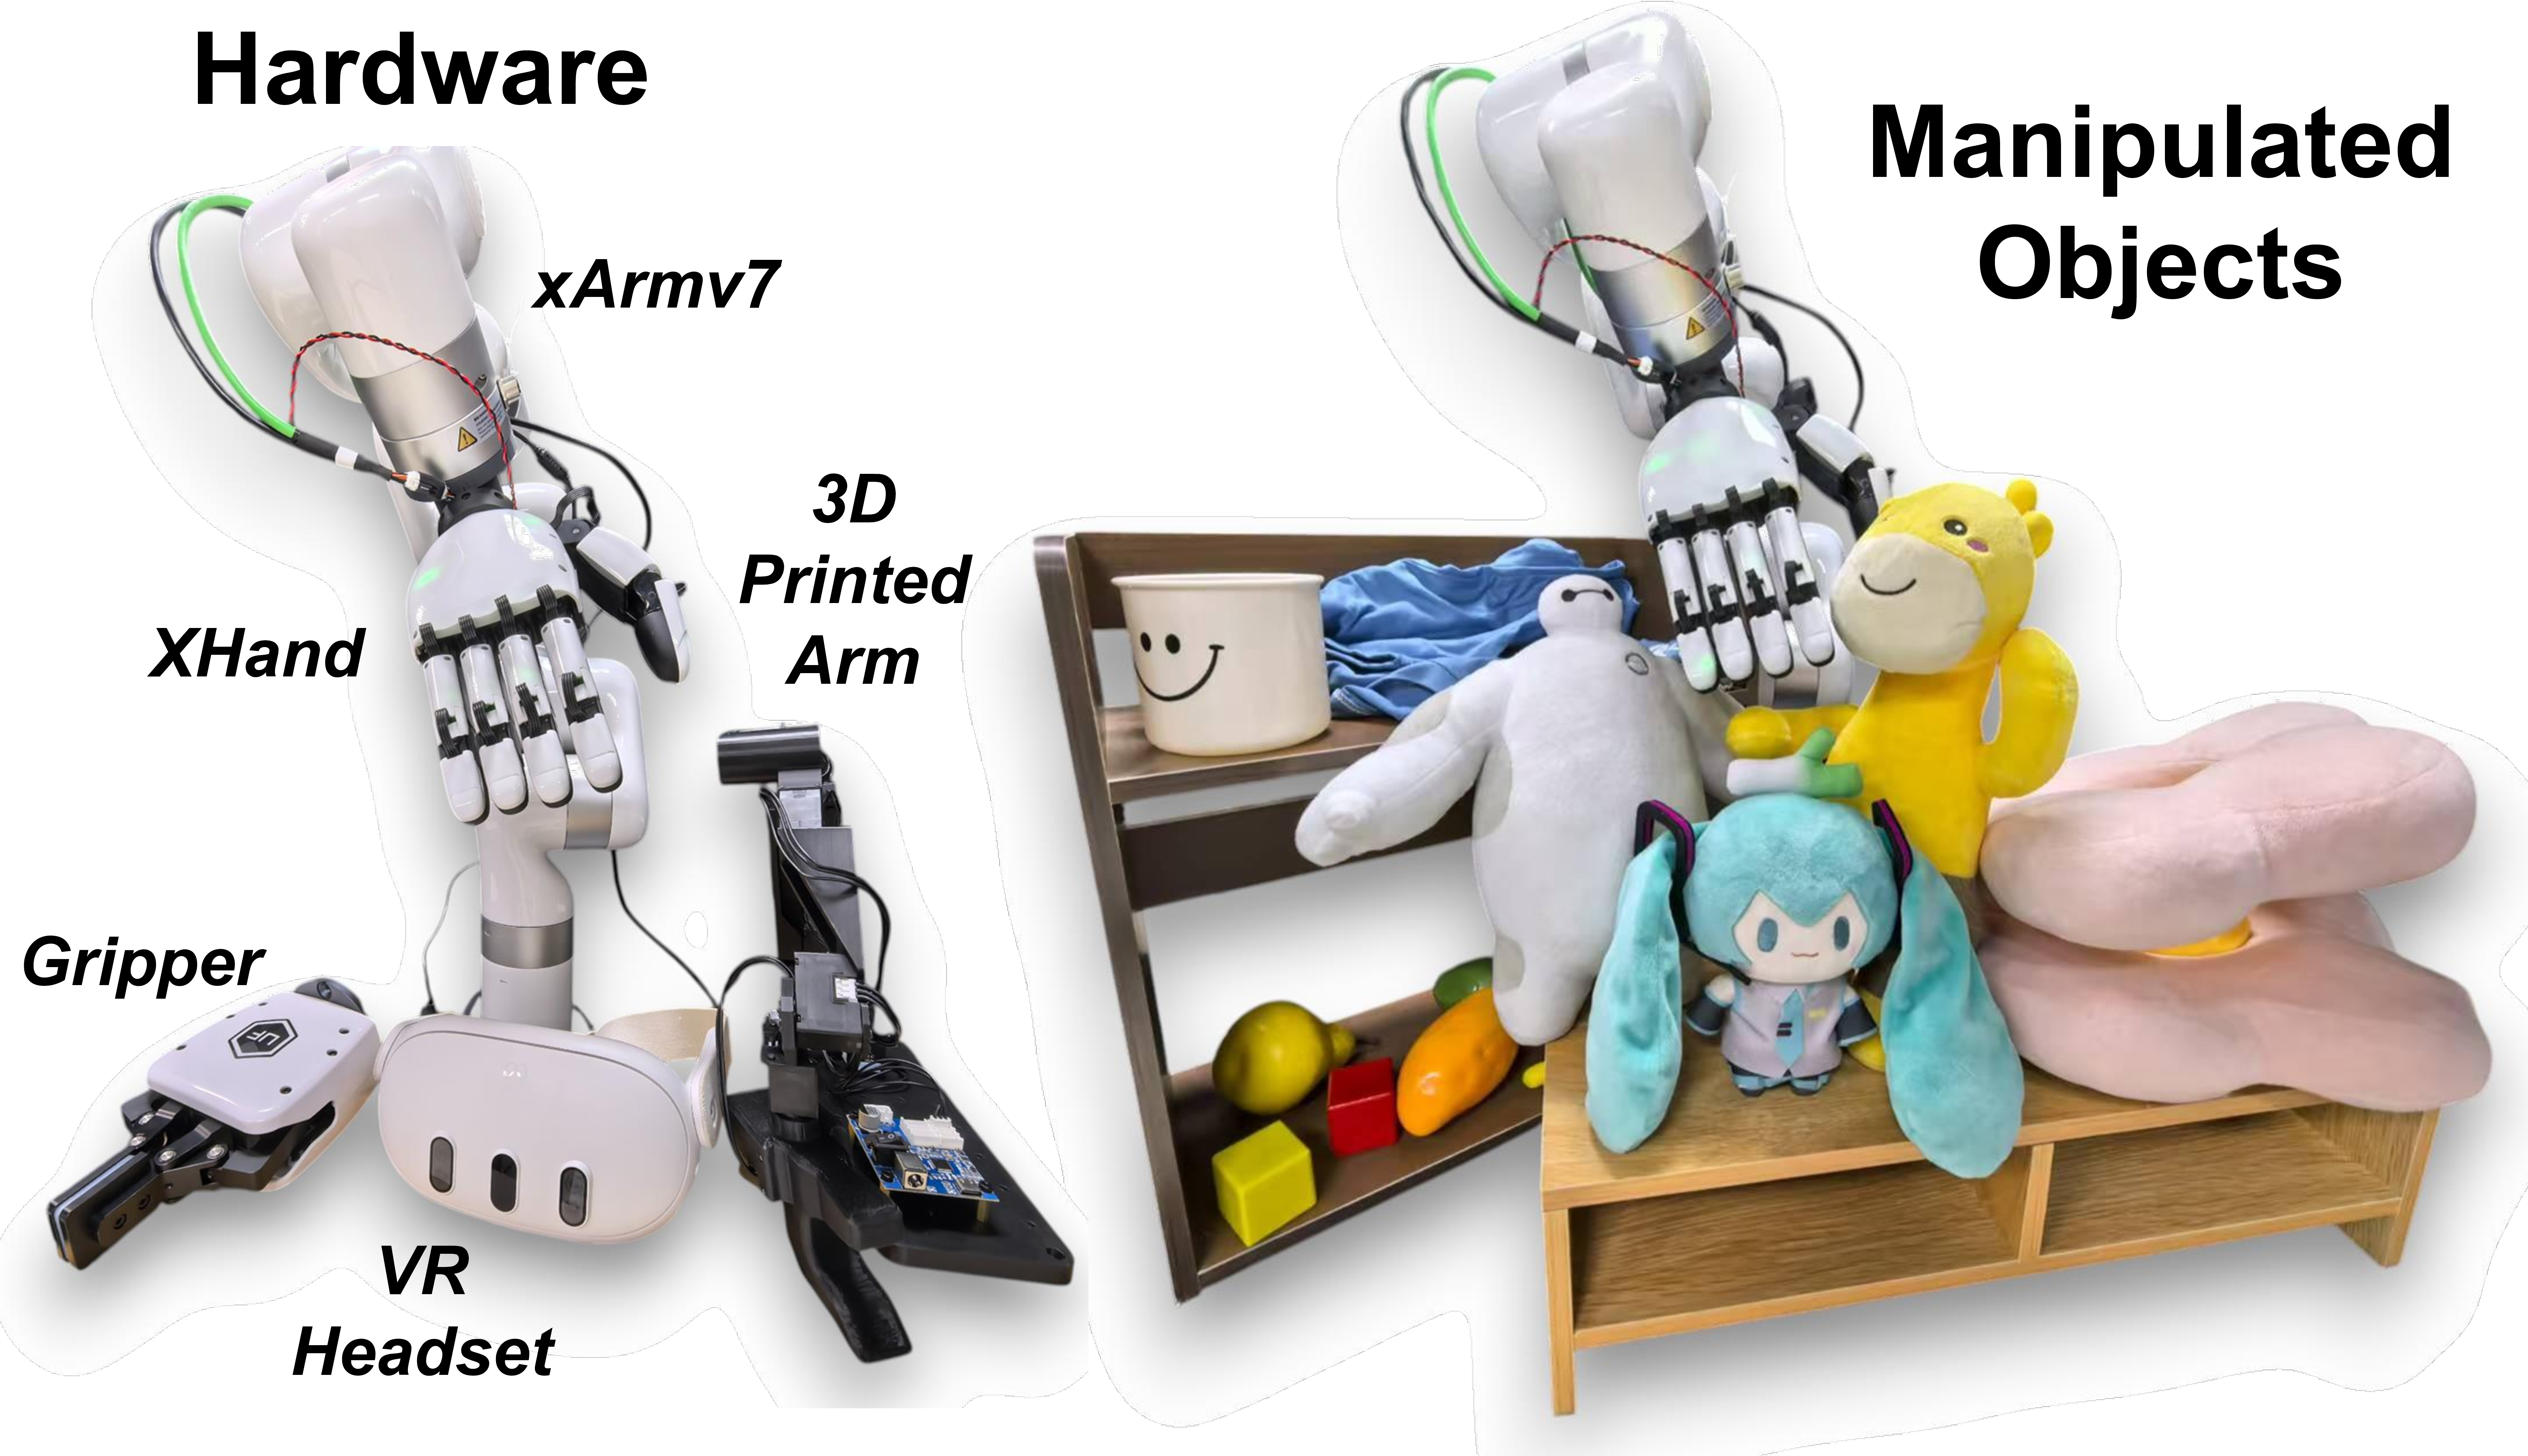
\includegraphics[width=\linewidth]{pics/real_setup.pdf}
  \vspace{-24pt}
  \caption{Hardware and manipulated objects used in real world experiments.}
  \vspace{-16pt}
  \label{fig:real_setup}
\end{wrapfigure}

\textbf{Hardware. }We evaluate our method on two single-arm hardware configurations commonly used in manipulation research: 
a) an UFACTORY xArm manipulator~\footnote{\url{https://www.ufactory.cc}} equipped with a two-finger parallel gripper, 
and b) an xArm paired with ROBOTERA XHand~\footnote{\url{https://www.robotera.com}} for dexterous manipulation. 
For visual sensing we use a third-person Intel RealSense L515 LiDAR camera that provides aligned color and depth frames. 
For the \textit{xArm + gripper} setup we additionally use a low-cost 3D-printed demonstration arm from GELLO~\citep{wu2024gello} as teleoperation device. For the \textit{xArm + XHand} setup, human hand motion is captured from a Meta Quest 3 headset and retargeted to the XHand. All computation runs on a single workstation equipped with an NVIDIA RTX 4090 laptop GPU. The robot and sensors are controlled over a local area network. 



\textbf{Teleoperation. }We collect demonstrations with two teleoperation pipelines. \textit{xArm + gripper} demonstrations are collected using the GELLO framework~\citep{wu2024gello}, a low-cost and intuitive teleoperation system that allows operators to demonstrate end-effector motions with a separate low-cost manipulator. \textit{xArm + XHand} demonstrations are recorded by capturing human hand kinematics via a Meta Quest 3 headset. The recorded wrist 6-DoF pose is mapped to the xArm end-effector via Inverse Kinematics (IK), finger joint values are retargeted to the XHand via AnyTeleop~\citep{qin2023anyteleop}.

% \subsection{Observation and Action Spaces}

\textbf{Observation and Action Spaces. }Visual input is the RGB-D stream from the RealSense L515. Frames are backprojected to form a colored point cloud. We convert each frame into a fixed-size point cloud by applying Farthest Point Sampling. 
Proprioceptive observations include the xArm joint angles. When the XHand is integrated, the observation space is extended to include the XHand’s joint angles as additional dimensions.
For the XHand configuration we additionally log tactile readings from fingertip sensors. All observations are normalized using the statistics computed on the training split. The policy outputs actions directly in joint space for both setups. We operate in absolute joint position control.

% \subsection{Baselines}

\textbf{Baselines. }We compare our method to two baselines. \textbf{Vanilla BC} processes observations through the same Observation Feature Extraction pipeline used by our method, and a 3-layer MLP is trained to regress actions in a standard behavior cloning setup~\citep{levine2016end}. \textbf{DP3}~\citep{ze20243d} is a diffusion-based generative policy operating on 3D point-cloud-conditioned actions. At inference DP3 employs DDIM~\citep{song2020denoising} denoising to obtain actions. Both baselines are trained on the identical demonstration sets and evaluated under the same closed-loop control as our method.

% \subsection{Tasks}

\textbf{Tasks. }We evaluate on tasks spanning low-DOF gripper control and high-DOF tactile dexterous manipulation. Low-DOF examples include a \textit{Pick Cube} task (gripper picks a cube from randomized table locations) and a \textit{Place Baymax} task (place a toy ``Baymax'' from table into a cabinet). High-DOF experiments use a 12-DOF dexterous hand equipped with tactile sensing and include contact-rich tasks such as \textit{Wipe Table} (multiple possible wiping contact points) and \textit{Place Toy Into Bin} (multiple candidate toy-boxes yielding multi-modal valid outcomes). For task like \textit{Place Baymax} we exploit a pretraining to fine-tuning regime. Models pretrained on a source task require substantially fewer target-task demonstrations to reach competitive performance.

% \subsection{Result Analysis}

\textbf{Result Analysis. }Our method consistently outperforms both baselines in success rate across low-DOF and high-DOF/tactile tasks (see Table~\ref{tab:real_result}). Qualitatively, Figure ~\ref{fig:real_compare} visualizes common failure modes of baselines, while our policy commits to coherent, single-mode rollouts when appropriate and preserves intra-mode variations elsewhere. Typical failure cases for our method occur at out-of-distribution object placements or when tactile sensing is intermittently noisy. These failures are rare and amenable to mitigation via modest additional demonstrations or data augmentation.

\vspace{-6pt}
\subsection{Ablations}
\vspace{-2pt}

\begin{figure*}[tb]
  \centering
  \includegraphics[width=0.99\linewidth]{pics/data_vis.pdf}
  \vspace{-8pt}
  \caption{Illustration of critical properties of \mymethod. (a) Action chunks are projected to 2D via PCA, colored by their assigned primary mode. (b) \mymethod’s one-step MeanFlow decoder achieves FPS comparable to 1-NFE DP3 while maintaining significantly higher success. (c) \mymethod{} preserves high success even with short chunks by avoiding primary mode bouncing.
  }
  \vspace{-8pt}
  \label{fig:data_vis}
\end{figure*}

\begin{figure*}[t]
  \centering
  
\includegraphics[width=0.99\linewidth]{pics/mode_vis.pdf}
  \vspace{-8pt}
  \caption{Visualization of the mode probability distribution predicted by the Primary Mode Policy $\pi_1$ at three selected frames. The vertical axis of the heatmap represents the mode index. 
  }
  \vspace{-16pt}
  \label{fig:mode_vis}
\end{figure*}


% We perform ablations to quantify the contributions of the two-stage design to study sensitivity to the discrete mode capacity and tokenization, to measure inference-budget trade-offs, and to evaluate how action-chunk length affects success and reactivity.


\textbf{Primary Mode and MeanFlow Ablation. }We ablate the two core components of our pipeline to establish their individual importance. First is to remove the Mode-conditioned MeanFlow Policy (MF) so that the system simply uses the Primary Mode Policy (PM)’s predicted VQ code and decodes it via the VQ-VAE reconstruction as the final action. Second is to remove the PM so that MF attempts to predict actions without being conditioned on a discrete mode. Results are reported in Table~\ref{tab:ablations}. Removing MF collapses performance almost completely, showing that a raw VQ reconstruction is insufficient as the final action when the number of modes is limited. The quantization error produces large reconstruction distortions that destroy task success. Conversely, removing PM yields a \(0.16\) absolute drop in success, which demonstrates that an explicit primary-mode selection substantially eases the downstream continuous generation problem and prevents coarse-mode bouncing. 


\textbf{Mode Capacity and Tokenization. }We study how the number of discrete primary modes $K$ and the choice of tokenization affect the PM learning and final task performance. We vary $K \in \{8, 64, 1024\}$ and compare VQ-VAE with a k-means tokenization baseline. Results appear in Table~\ref{tab:ablations}. A small $K$ helps the PM to learn, but it risks underfitting when the task’s action-chunk distribution is complex. Large $K$ increases expressivity but makes the PM hard to learn. In our domains the trade-off is modest and $K=64$ achieves a good balance across tasks. Different tokenizers produce similar final success rates, suggesting the approach is robust to discretization methods. Our method mainly needs a reasonable set of coarse modes rather than a specific quantizer. To further illustrate mode structure we project action-chunks into 2D (PCA) and color by assigned mode. The visualization shows clear coarse-mode clusters on the action manifold, as visualized in Figure~\ref{fig:data_vis} (a). We also visualize the policy's outputs at different timesteps (see Figure~\ref{fig:mode_vis}).
For a more detailed qualitative analysis of the primary mode policy's behavior, see Appendix.

\begin{wraptable}{r}{0.45\textwidth}  
  \centering 
  \vspace{-4pt}
  \begin{tabular}{l c c}  
    \toprule  
    Variations & ODE Solver & Success \\ 
    \midrule  
    CFM    & 1-NFE Euler    & \dd{0.69}{0.03} \\
    CFM    & 10-NFE Euler    & \dd{0.69}{0.02} \\
    CFM    & Runge-Kutta    & \dd{0.68}{0.01} \\
    Meanflow    & 1-NFE    & \ddbfgreen{0.72}{0.02} \\
    \bottomrule  
  \end{tabular}
  \vspace{-4pt}
    \caption{Comparison of success for MeanFlow (MF) and Conditional Flow Matching (CFM), varying the ODE solver and NFE.} 
    \vspace{-8pt}
  \label{tab:meanflow}  
\end{wraptable}


\textbf{Ablation on Meanflow. }This ablation aims to evaluate the performance difference between MeanFlow and Conditional Flow Matching (CFM)~\citep{lipman2022flow}, where CFM is tested under different Ordinary Differential Equation (ODE) numerical integration methods. Though CFM theoretically defines a constant velocity field when mapping from noise to target distribution, the parameterized neural network introduces nonlinearity in numerical computations. This makes the exploration of diverse ODE integrators non-trivial. For Runge-Kutta integration, we adopt the Dormand-Prince 5 method, a widely used choice for adaptive-stepsize ODE solving. As shown in Table~\ref{tab:meanflow}, varying ODE numerical integrators yields negligible performance improvements for CFM. In contrast, replacing CFM with MeanFlow results in a performance gain.


% \subsection{Speed–Accuracy Trade-off}

\textbf{Speed–Accuracy Trade-off. }We examine how the number of function evaluations (NFE) during inference affects both inference speed and success. We compare our one-step MeanFlow decoder to DP3 at different NFE settings, plots are in Figure~\ref{fig:data_vis} (b).  Our one-step generator achieves inference speed comparable to DP3 with 1-NFE while delivering substantially higher success. More generally, we observe that within the tested range the total NFE has a surprisingly small influence on success, which suggests that for these simulated tasks the NFE is not the dominant bottleneck. We hypothesize this limited sensitivity is due to the tasks’ tolerance to small action perturbations in simulation. 
% Whether the same holds for high-precision or contact-sensitive, real world tasks needs further study.


\textbf{Action-chunk Length and Reactivity. }All experiments here are conducted on real settings described in the Real World Evaluation section. We sweep action-chunk length and measure success. Shorter chunks make the controller more open-loop reactive and therefore better able to respond to unexpected environment changes. However, short chunks also tend to increase trajectory jitter and occasional stoppages. Our method maintains relatively high success even at short chunk lengths, showing the two-stage design preserves primary-mode consistency while allowing rapid reactivity. Results appear in Figure~\ref{fig:data_vis} (c).

\vspace{-4pt}
\subsection{Failure Cases and Limitations}
\vspace{-2pt}

While \mymethod{} demonstrates strong performance across a wide range of manipulation benchmarks, it has two notable limitations. First, because primary-mode selection operates on discretized action chunks, the method exhibits reduced temporal granularity in very high-dynamics, low-latency tasks. Second, the discrete codebook introduces a trade-off between expressivity and learnability. Larger \(K\) improves representational capacity but makes primary-policy learning harder, while smaller \(K\) constrains diversity. We address this in the paper via targeted ablations and validation sweeps. Promising directions to reduce per-task tuning include shared or meta-learned codebooks, end-to-end distillation, and multi-task pretraining to improve generalization and reduce pipeline overhead.




